\blankpage

\newwatermark[pagex={5}]{\vspace{2.5cm}\hspace*{7.8cm}
\includegraphics[scale=1]{../watermarks/1modulo9ano.pdf}}

\chapter{1. Práticas corporais: dos jogos eletrônicos até aos esportes radicais}

\vspace*{-2\baselineskip}

\coment{Habilidades da BNCC: EF67EF01, EF67EF06, EF89EF03, EF89EF15, 
EF89EF18}

\colorsec{Habilidades do SAEB}

\begin{itemize}
\item
  Identificar as diferentes valências físicas necessárias
  à realização de práticas corporais (jogos eletrônicos, lutas, práticas
  corporais de aventura, ginásticas, esportes e dança).
\item
  Identificar o valor do patrimônio urbano e natural nas vivências das
  práticas corporais de aventura urbana e na natureza.
\item
  Identificar as características (códigos, rituais, elementos
  técnico-táticos, indumentária, materiais, instalações, instituições)
  das lutas.
\item
  Analisar as práticas corporais frente à disponibilidade de locais para
  sua vivência.
\item
  Analisar as transformações históricas, o processo de esportivização e
  a midiatização das práticas corporais, com ênfase nas lutas.
\end{itemize}

\reversemarginpar\marginnote{O objetivo deste módulo é habilitar o
estudante a entender o processo de esportivização e identificar as práticas
corporais presentes na sociedade, reconhecendo suas principais
características, e as valências físicas presentes nas
modalidades esportivas.\\}

\conteudo{As práticas corporais (jogos eletrônicos, ginásticas esportes, lutas,
danças etc.) são manifestações corporais presentes na sociedade. Em cada uma dessas atividades são trabalhadas as \textbf{valências físicas}, que são: \textbf{força} (vencer uma
carga externa), \textbf{velocidade} (realizar um movimento no menor
tempo possível), \textbf{resistência} (realizar o mesmo movimento por
vários segundos) e \textbf{flexibilidade} (capacidade de esticar uma
musculatura ao máximo).

Além disso, muitas práticas passam por um processo de \textbf{esportivização}, ou
seja, deixam de ser uma atividade voltada para o lazer e passam a ser um
esporte oficial. Suas características são:

\begin{itemize}
\item
  Presença de regras oficiais padronizadas;
\item
  Criação de órgãos oficiais para fiscalizar o esporte (federação e
  confederação);
\item
  Competições oficiais e treinamentos específicos.
\end{itemize}
}

\colorsec{Atividades}

\num{1} Escreva as capacidades físicas mais utilizadas em cada prática corporal:

\begin{escolha}
\item
  Corrida dos 100 metros: \coment{velocidade.}
\item
  Maratona: \coment{resistência.}
\item
  Ginástica artística: \coment{flexibilidade.}
\item
  Levantamento olímpico: \coment{força.}
\end{escolha}

\coment{Por meio desta atividade, o estudante vai
poder relacionar e identificar as capacidades físicas utilizadas em
algumas práticas corporais.}

\num{2} Relacione o tipo de práticas corporais de aventura (urbana ou
  natureza) com as modalidades apresentadas a seguir.

\begin{multicols}{2}

(\coment{1}) Slackline

(\coment{2}) Moutain bike

(\coment{2}) Corrida de orientação

(\coment{1}) Skate

\columnbreak

(1) Prática de aventura urbana

(2) Prática de aventura na natureza

\end{multicols}

\coment{O objetivo desta atividade é habilitar o estudante a
distinguir as práticas corporais realizadas nos ambientes urbanos das que 
ocorrem na natureza, valorizando os espaços para essas modalidades.}

\num{3} Observe a imagem a seguir:

\begin{figure}[htpb!]
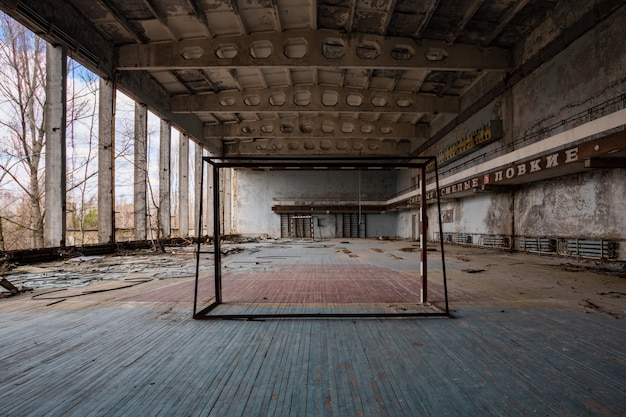
\includegraphics[width=2.99444in,height=1.99477in]{./imgs/img1.jpg}
\caption{Fonte: https://br.freepik.com/fotos-gratis/ginasio-abandonado-em-pripyat\_13499703.htm\#query=parque\%20abandonado\&position=6\&from\_view=search\&track=ais}
\end{figure}

Observando a imagem, é possível realizar alguma prática corporal? Qual é
o nosso dever em relação a esses espaços.

\linhas{3}

\coment{Na imagem, observa-se um ginásio esportivo abandonado, de
infraestrutura comprometida, cujo abandono, além de oferecer riscos
à saúde dos esportistas, inviabiliza o uso pela comunidade. O papel
das pessoas é preservar espaços públicos como esse, que podem ser 
extremamente benéficos quando adequadamente utilizados.
O propósito desta atividade é estimular o espírito crítico 
dos estudantes no que concerne aos espaços públicos disponíveis
na cidade.}

\num{4} No passado, o judô era uma luta voltada para a defesa pessoal.
  Atualmente é uma modalidade olímpica dividida em categorias, com 
  distinção de golpes proibidos e legítimos. É possível afirmar que essa
  luta passou por um processo de esportivização? Justifique sua
  resposta.

  %É adequado chamar o judô de "luta"? Minha experiência em escolas me ensinou que a expressão "arte marcial" é mais adequada (mas pode ser ignorância minha). (Rogério, 6/4/23, 13h08)

\linhas{3}

\coment{É correto afirmar que o judô passou pelo processo de
esportivização, pois, embora tenha sido um luta voltada para a autodefesa,
hoje em dia é um esporte com categorias, regras e golpes padronizados,
que são realizados em competições oficiais, como as Olimpíadas.

O objetivo dessa atividade é que o estudante
compreenda o processo por meio do qual uma prática corporal se torna 
um esporte oficial.}

\colorsec{Treino}

\num{1} Observe a imagem a seguir:

\begin{figure}[htpb!]
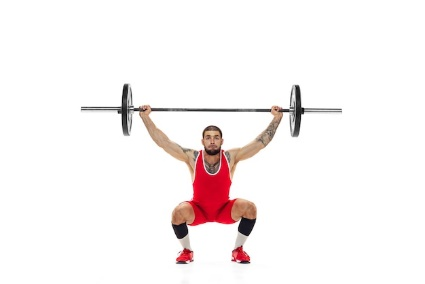
\includegraphics[width=1.92222in,height=1.28367in]{./imgs/img2.jpg}
\caption{Disponível em:
https://br.freepik.com/fotos-gratis/jovem-esportivo-treinando-com-barra-de-peso-isolada-sobre-fundo-de-estudio-branco-situps\_24908397.htm\#query=levantamento\%20de\%20peso\&position=41\&from\_view=search\&track=ais}
\end{figure}

Com base na imagem, o atleta está praticando uma modalidade que trabalha
a valência física de

\begin{escolha}
\item força, pois está vencendo uma carga externa que são as anilhas.

\item resistência, pois ficar agachado exige contração muscular das pernas.

\item velocidade, pois deve-se pegar a barra no chão e levantá-la para
cima.

\item flexibilidade, pois os músculos dos braços estão esticados.
\end{escolha}

\coment{SAEB: Identificar as diferentes valências físicas necessárias à
realização de práticas corporais (jogos eletrônicos, lutas, práticas
corporais de aventura, ginásticas, esportes e dança).

BNCC: EF67EF06 - Analisar as transformações na organização e na prática
dos esportes em suas diferentes manifestações (profissional e
comunitário/lazer).

a) Correta. de fato, a valência física trabalhada pelo atleta da imagem 
é a força, porque ele está vencendo uma caga externa composta por anilhas
e barra.
b) Incorreta. O levantamento olímpico trabalha a força, não a
resistência.
c) Incorreta. A velocidade não é praticada nesse esporte.
d) Incorreta. Nesse esporte, a flexibilidade não é priorizada.}

\num{2} Leia o texto a seguir:

\begin{quote}
O município de Salvaterra, no arquipélago paraense do Marajó, será palco
da estreia da luta marajoara nos Jogos Estudantis Paraenses (Jeps).

{[}...{]}

A típica luta marajoara é um combate corpo a corpo, que tem o objetivo
de projetar o oponente de costas ao chão e dominá-lo, esporte semelhante
ao Wrestling, praticado no norte do Brasil. Esta é a primeira vez que a
modalidade é incluída no torneiro, que está na sua 62ª edição.

\fonte{GE Pará. Salvaterra recebe os primeiros combates da luta marajoara
como modalidade do Jeps. Disponível em:
https://ge.globo.com/pa/noticia/salvaterra-recebe-os-primeiros-combates-da-luta-marajoara-como-modalidade-do-jeps.ghtml
. Acesso em: 6 abr. 2023.}
\end{quote}

Com base no texto, pode-se afirmar que a luta marajoara passou
por um processo de esportivização porque

\begin{escolha}
\item foram criados órgão oficiais relacionados a essa prática.

\item a prática está presente em um evento oficial.

\item o objetivo da prática foi alterado para a competição.

\item essa prática se assemelha à de um outro esporte.
\end{escolha}

\coment{SAEB: Analisar as transformações históricas, o processo de
esportivização e a midiatização das práticas corporais, com ênfase nas
lutas.

BNCC: EF89EF18 - Discutir as transformações históricas, o processo de
esportivização e a midiatização de uma ou mais lutas, valorizando e
respeitando as culturas de origem.

a) Incorreta. Não há alusão, no texto, à criação de
federações ou confederações da luta marajoara. 
b) Correta. A luta marajoara faz parte de um evento oficial de
competição, os Jogos Estudantis Paraenses.
c) Incorreta. Não há alusão, no texto, à alteração do objetivo da luta
marajoara. 
d) Incorreta. A semelhança entre a luta marajoara e o
wrestling não define essa prática corporal como esporte.}

\num{3} Leia o texto a seguir:

\begin{quote}
Skatistas de Curitiba terão, em breve, um novo espaço para praticar o
esporte. A Prefeitura de Curitiba começará a construir nos próximos 15
dias a maior pista pública de skate da cidade 

A pista, de 450 metros quadrados, será a primeira da região e é uma antiga 
reivindicação da população. O projeto feito pela Secretaria Municipal do 
Meio Ambiente teve a participação de skatistas. "Tomamos os cuidado de 
ouvir os praticantes do esporte e deixar o projeto o mais próximo possível 
da necessidade dos usuários", conta o superintende de obras e serviços da 
secretaria, Paulo Dalmaz.

%Felipe: consultei o original e alterei o trecho do texto escolhido. Na questão originla, a alternativa correta estava baseada em uma inferência duvidosa; entendo que, agora, a questão ficou mais consistente, além de enfatizar a demanda da população pelo esporte. (Rogério, 6/4/23, 13h45)

\fonte{Prefeitura Municipal de Curitiba. Nova pista pública de skate
será a maior da cidade. Disponível em:
https://www.curitiba.pr.gov.br/noticias/nova-pista-publica-de-skate-sera-a-maior-da-cidade/7410. Acesso em: 6 abr. 2023.}
\end{quote}

Após a leitura do texto, pode-se afirmar que o objetivo da construção da 
pista pública de skate é

\begin{escolha}
\item formar novos atletas para competições oficiais.

\item incentivar o uso de um novo meio de transporte.

\item atender à demanda da população pela prática do skate.

\item criar novos investimentos financeiros para a prefeitura.
\end{escolha}

\coment{SAEB: Identificar o valor do patrimônio urbano e natural
nas vivências das práticas corporais de aventura urbana e na natureza.

BNCC: EF67EF06 - Analisar as transformações na organização e na prática
dos esportes em suas diferentes manifestações (profissional e
comunitário/lazer).

a) Incorreta. Não há alusão, no texto, ao propósito de formar novos
atletas.
b) Incorreta. Não há alusão, no texto, ao uso do skate como meio
de locomoção. 
c) Correta. O segundo parágrafo é explícito quanto à demanda da 
população por um espaço adequado para a prática do esporte.
d) Incorreta. Não há alusão, no texto, ao propósito de criação de novos investimentos da prefeitura.}

\chapter{2. Esporte e dança}

\coment{O objetivo deste módulo é que o aluno compreenda as definições dos
esportes e entenda as características das danças, especificamente das
danças urbanas.\\

Habilidades da BNCC: EF67EF12, EF67EF13.}

\colorsec{Habilidades do SAEB}

\begin{itemize}
\item
  Diferenciar os esportes com base nos critérios de sua lógica interna.
\item
  Diferenciar as danças urbanas, seus elementos constitutivos e seu
  valor cultural nas demais manifestações da dança.
\end{itemize}

\conteudo{As \textbf{danças urbanas} desenvolveram-se em centros
urbanos ou periferias como forma de expressão e crítica social, por meio
do uso do corpo. É o caso da cultura do hip-hop, que abarca traços
de diversas culturas e traz muitos benefícios para o praticante.

Além disso, muitas dessas danças, como o \textbf{breaking}, estão passando
pelo processo de esportivização e vão fazer parte de eventos oficiais,
como as Olimpíadas.}

\colorsec{Atividades}

\num{1} Relacione os elementos do hip-hop (primeira coluna) com suas respectivas características (segunda coluna).

\begin{multicols}{2}

(1) Rap

(2) Breaking

(3) Grafite

(4) DJ

\columnbreak

(\rosa{2}) Dança do hip-hop em que o dançarino pode improvisar os movimentos.

(\rosa{3}) Desenhos artísticos feitos em muros ou em paredes com spray.

(\rosa{1}) Canção do hip-hop que tem improvisações e rimas.

(\rosa{4}) Pessoa responsável pela mixagem do som.
\end{multicols}

\coment{ O objetivo dessa atividade é que o aluno
identifique os elementos da cultura do hip-hop.}

\num{2} Observe a imagem a seguir:

\begin{figure}[htpb!]
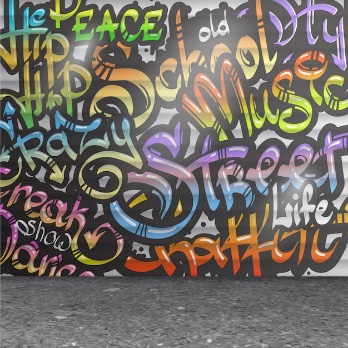
\includegraphics[width=1.57407in,height=1.57407in]{./imgs/img3.jpg}
\caption{Fonte: https://br.freepik.com/vetores-gratis/fundo-da-parede-de-graffiti\_4631697.htm\#page=2\&query=hip-hop\&position=47\&from\_view=search\&track=sph}
\end{figure}

Podemos dizer que a imagem mostra uma pichação? Justifique sua resposta.

\linhas{4}

\coment{Na imagem, observa-se não uma pichação, mas um grafite. 
O grafite é uma forma de arte visual cujos desenhos são feitos com spray,
normalmente realizados com autorização de prefeituras ou donos de
estabelecimentos. As pichações, por sua vez, são formas de vandalismo.}

%Felipe: acredito que a distinção entre grafite e pichação explicada no gabarito é, para dizer o mínimo, simplória. Além disso, deixa espaço aberto para nosso material ser alvo de duras críticas. Há quem defenda a pichação como forma de expressão. 

\num{3}  Marque com um X as danças que são consideradas como esportes oficiais.

\begin{boxlist}
\item Breaking. \coment{X}

\item Dança esportiva. \coment{X}

\item Maculelê.

\item Toré.
\end{boxlist}

\coment{O propósito desta atividade é facultar ao estudante a compreensão 
de que muitas danças podem ser consideradas como esporte oficial.}

\num{4}  Relacione as danças a seguir com suas respectivas origens.

\begin{multicols}{2}
(\coment{3}) Tango.

(\coment{1}) Hip-hop.

(\coment{2}) Samba.

(\coment{4}) Dança esportiva

\columnbreak

(1) Dança urbana.

(2) Dança afro-brasileira.

(3) Dança de salão.

(4) Dança olímpica.
\end{multicols}

\coment{O objetivo dessa atividade é que o estudante identifique as
danças e sua origem.}

\num{5} Redija um texto curto explicando a origem da cultura hip-hop
nas periferias das cidades dos Estados Unidos.

\linhas{4}

\coment{O hip-hop surgiu nos guetos e bairros pobres dos Estados
Unidos como forma de protesto contra o racismo e a exclusão social.
Noos gêneros de canção, como o rap, de dança, como o break, e de artes 
visuais, como o grafite, eram formas de expressão da denúncia e das 
críticas dessa geração de artistas. 

O objetivo desta atividade é que aluno compreenda o contexto em que se 
originou a cultura hip-hop.}

\colorsec{Treino}

\num{1} Leia a reportagem a seguir.

\begin{quote}
A revolução está aqui! Em Paris 2024, o breaking fará sua
estreia no programa dos Jogos Olímpicos. {[}...{]}

Serão três competições nas quais os atletas poderão garantir uma vaga
para a estreia do breaking em Paris 2024: o Mundial de 2023, os
jogos/campeonatos continentais e a série de classificatórios olímpicos.
{[}...{]}

Haverá dois eventos de breaking em Paris 2024 --- as competições
individuais masculina e feminina. Em cada um, 16 B-Boys e 16 B-Girls
lutarão para avançar para as próximas rodadas (ou pela medalha de ouro
na final) em batalhas solo cara a cara.

\fonte{Olympics. Rumo a Paris 2024: confira o sistema da classificação Olímpica do
breaking. Disponível em:
https://olympics.com/pt/noticias/sistema-de-classificacao-breaking-jogos-olimpicos-paris-2024.
Acesso em: 6 abr. 2023.}
\end{quote}

Considerando as informações do texto, pode-se afirmar que a dança citada
é esporte oficial porque

\begin{escolha}
\item prevê disputas por medalhas olímpicas.

\item fez parte das edições olímpicas anteriores.

\item inclui participação de homens e mulheres.

\item ter eventos de competições esportivas.
\end{escolha}

\coment{SAEB: Diferenciar os esportes com base nos critérios de sua lógica
interna.

BNCC: EF67EF12 - Planejar e utilizar estratégias para aprender elementos
constitutivos das danças urbanas.

a) Incorreta. A disputa por medalhas olímpicas não caracteriza se uma
modalidade é um esporte oficial ou não.
b) Incorreta. A dança urbana não foi modalidade esportiva de olimpíadas 
anteriores. A estreia ocorrerá em 2024.
c) Incorreta. A participação de homens e mulheres não caracteriza o
breaking como esporte oficial.
d) Correta. No texto, afirma-se que, além das Olimpíadas, os atletas
devem participar de outras competições oficiais.}

\num{2} Leia o texto a seguir.

\begin{quote}
A cultura Hip Hop é formada pelos seguintes elementos: o rap, o graffiti
e o break. {[}...{]}

Os três elementos juntos compõem a cultura hip hop, que muitos dizem que
é a ``CNN da periferia'', ou seja, que o hip hop seria a única forma da
periferia, dos guetos expressarem suas dificuldades, suas necessidades
de classes excluídas.

\fonte{Secretaria da Educação do Paraná. Dança de Rua. Disponível em:
http://www.educacaofisica.seed.pr.gov.br/modules/conteudo/conteudo.php?conteudo=60.
Acesso em: 6 abr. 2023.}
\end{quote}

Com base no texto, o hip-hop surgiu como forma de

\begin{escolha}
\item expressão de adversidades.

\item incentivo à prática da dança.

\item criação de nova modalidade de dança.

\item assistência social do governo.
\end{escolha}

%Tive de alterar a primeira alternativa. O problema desta questão é o seguinte: o autor do material insiste no caráter de protesto do hip-hop, mas o texto fala em expressão de dificuldades e necessidades. Protesto e expressão se aproximam, se tocam, mas não saõ necessariamente a mesma coisa. O problema é que o texto escolhido não diz o que o autor quer que ele diga. 

\coment{SAEB: Diferenciar as danças urbanas, seus elementos constitutivos
e seu valor cultural nas demais manifestações da dança.

BNCC: EF67EF13 - Diferenciar as danças urbanas das demais manifestações
da dança, valorizando e respeitando os sentidos e significados
atribuídos a eles por diferentes grupos sociais.

a) Correta. De acordo com o texto, no hip-hop o rap, o grafite e
o break são formas de expressão das dificuldades dos moradores da 
periferia.
b) Incorreta. A origem do hip-hop está mais associada à expressão das 
adversidades das pessoas da periferia do que ao incentivo à dança.
c) Incorreta. A origem do hip-hop está mais associada à expressão das 
adversidades das pessoas da periferia do que à criação de uma nova
modalidade de dança.
d) Incorreta. Não há, no texto, referências ao hip-hop como forma de 
assistência social do governo.}

\num{3}  Leia a reportagem a seguir.

\begin{quote}

Entre os ritmos apresentados, um que causou bastante animação na plateia
foi a performance de k-pop, gênero originário da Coreia do Sul, que
agrega elementos do pop, rock, hip-hop, rap, reggae, street dance e
outras sonoridades contemporâneas.

\fonte{Notícias do Acre. Escola de Música do Acre e Balancé Balé promovem atividades de dança com
a comunidade. Disponível em:
https://agencia.ac.gov.br/escola-de-musica-do-acre-e-balance-bale-promovem-atividades-de-danca-com-a-comunidade/.
Acesso em: 21 fev. 2023.}
\end{quote}

Considerando a leitura do texto, é possível inferir que o k-pop pode ser
considerado como dança urbana por

\begin{escolha}
\item ter origem asiática.

\item ser realizado em grupos.

\item basear-se em movimentos corporais.

\item ter forte influência do hip-hop.
\end{escolha}

\coment{SAEB: Diferenciar as danças urbanas, seus elementos constitutivos
e seu valor cultural nas demais manifestações da dança.

BNCC: EF67EF13 - Diferenciar as danças urbanas das demais manifestações
da dança, valorizando e respeitando os sentidos e significados
atribuídos a eles por diferentes grupos sociais.

a) Incorreta. A origem asiática do k-pop não implica que essa modalidade
seja considerada dança urbana.
b) Incorreta. A prática da dança em grupo não tem relação com sua
classificação com dança urbana.
c) Incorreta. Os movimentos corporais são constitutivos de quaisquer 
danças, de modo que essa característica não é suficiente para caracterizar 
o hip-hop como danças urbanas.
d) Correta. O k-pop se inspirou em elementos do hip-hop, como os
movimentos de dança do break e o rap.}

\chapter{3. Esporte na mídia}

\coment{O objetivo deste módulo é habilitar o estudante à análise 
crítica da presença do doping e da corrupção, em eventos esportivos, 
e à compreensão da mídia com padronizadora do corpo e consequentemente 
da saúde das pessoas.\\
Habilidades da BNCC: EF89EF08, EF89EF09.}

\colorsec{Habilidades do Saeb}

\begin{itemize}
\item
  Avaliar a multiplicidade de padrões de estética corporal disseminados
  pela mídia, que geram uma prática excessiva de exercícios e o uso de
  recursos ergogênicos.
\item
  Avaliar os problemas presentes nos esportes e abordados pela mídia,
  tais como doping, violência ou corrupção.
\item
  Avaliar a relação entre as práticas corporais e a promoção da saúde.
\end{itemize}

\conteudo{Os esportes são manifestações corporais presentes na sociedade.
Trata-se de práticas que trazem inúmeros benefícios a saúde física e 
mental das pessoas, como controle da massa corporal, socialização e
prevenção ao estresse. Porém, por causa de diversos motivos, como a ampla
cobertura da mídia e dos contratos milionários a ela relacionados, existem
pessoas que procuram obter resultados a qualquer custo, recorrendo a
práticas ilícitas como o doping e a corrupção.

Além disso, a mídia contribui para o discurso de padronização do corpo, 
ou seja, reproduz ideais de ``corpo perfeito e saudável'' que as 
pessoas, supostamente, deveriam ter. Essa busca incessante por um
modelo de perfeição, ao qual a maioria das pessas não corresponde,
é uma das causas de transtornos alimentares, como a bulimia.}

\colorsec{Atividades}

\num{1}  Relacione o nome dos transtornos alimentares com suas respectivas características.

\begin{multicols}{2}

(1) Anorexia.

(2) Bulimia.

(3) Vigorexia.

(4) Ortorexia.

\columnbreak

(\rosa{3}) Pessoa que se enxerga com baixa massa muscular.

(\rosa{4}) Pessoa que se preocupa exageradamente com a alimentação saudável.

(\rosa{1}) Pessoa que se enxerga com obesidade.

(\rosa{2}) Pessoa que induz o vômito.
\end{multicols}

\coment{O objetivo desta atividade é que o estudante reconheça e
identifique os principais transtornos alimentares que existem.}

\num{2} As competições, como as Copas do Mundo e as Olimpíadas, são
eventos esportivos que estão presentes na mídia, devido a altos
investimentos financeiros de governos e empresas privadas.
Consequentemente, há atletas que fazem de tudo para obter sucesso, 
incluindo práticas de corrupção e o uso de doping. Dessa maneira, 
escreva as definições desses dois problemas nos esportes.

\linhas{4}

\coment{No esporte, a \textbf{corrupção} corresponde à manipulação de
resultados por meio de recursos financeiros. O \textbf{doping} é o uso
de suplementos e anabolizantes ilegais para melhorar o condicionamento 
físico e, consequentemente, os resultados do atleta.

Por meio dessa atividade o estudante pode entender de maneira crítica 
alguns problemas presentes nos esportes no âmbito competitivo.}

\num{3} É de senso comum que qualquer prática esportiva traz benefícios 
para a saúde física e mental, como o fortalecimento muscular e a
socialização. Entretanto, é preciso conhecer o benefício específico de
cada esporte. Dessa maneira, relacione os esportes a seguir com seus 
principais benefícios.

\begin{multicols}{2}
(1) Pilates.\medskip

(2) Treinamento resistido.\medskip

(3) Natação.\medskip

(4) Corrida de 100 metros.

\columnbreak

(\coment{4}) Ajuda na capacidade física de velocidade.

(\coment{1}) Melhora a flexibilidade.

(\coment{2}) Aumento de massa magra.

(\coment{3}) Aumento da capacidade cardiovascular.
\end{multicols}

\coment{O propósito desta atividade é habilitar o estudante a
identificar e analisar os benefícios específicos de cada uma 
das práticas corporais.}

\num{4}  Observe a imagem a seguir:

\begin{figure}[htpb!]

\includegraphics[width=4.07407in,height=2.28999in]{./imgs/img4.jpg}
\caption{Fonte: https://br.freepik.com/psd-gratuitas/modelo-de-facebook-de-treinamento-de-musculacao-de-design-plano\_35720255.htm\#query=propaganda\%20academia\&position=16\&from\_view=search\&track=ais}
\end{figure}

Se essa propaganda de academia fosse apresentada no Brasil, ia ter uma
representatividade? Justifique sua resposta.

\linhas{4}

\coment{Resposta: Não, pois os corpos apresentados em propagandas (mídias) não
representam a maioria da população brasileira. Pelo fato que a mídia
padroniza o mesmo tipo de corpo: um corpo alto, magro, definido, branco
e sem imperfeições na pele.

Orientação para o professor: Por meio dessa atividade o estudante vai
analisar e entender de maneira crítica como a mídia padroniza um
determinado padrão corporal que muitas vezes não existe. Habilidade
Saeb: Avaliar a multiplicidade de padrões de estética corporal
disseminados pela mídia, que geram uma prática excessiva de exercícios e
o uso de recursos ergogênicos.}

\colorsec{Seção Treino}

\num{1} Leia o texto a seguir:

\begin{quote}
Comer é, sem dúvida, um dos prazeres da vida. Porém, quando a ingestão
de alimentos passa dos limites, o que deveria ser prazeroso torna-se um
pesadelo, que pode intervir diretamente na saúde física e mental do
indivíduo. {[}...{]}

{[}...{]} a pessoa também apresenta episódios de compulsão alimentar,
mas após estes momentos tem tanto medo de ganhar peso que acaba
adquirindo métodos para compensar e evitar o ganho de massa, como
vômitos, uso de laxantes, exercícios físicos em exagero e uso de
diuréticos''.

\fonte{Especialista orienta como identificar e tratar transtornos alimentares.
Secretária da Saúde do Estado do Ceará. Disponível em:
https://www.saude.ce.gov.br/2019/09/05/especialista-orienta-como-identificar-e-tratar-transtornos-alimentares/.
Acesso em: 22 fev. 2023.}
\end{quote}

O texto mostra um transtorno alimentar que é

\begin{escolha}
\item a bulimia, que é a pessoa realizar ações maléficas após comer algo.

\item a anorexia, que é comer excessivamente durante o dia.

\item a vigorexia, que é desejo de aumentar o volume muscular.

\item a ortorexia, que é a pessoa usar diferentes medicamentos.
\end{escolha}

\coment{Saeb: Avaliar a multiplicidade de padrões de estética corporal
disseminados pela mídia, que geram uma prática excessiva de exercícios e
o uso de recursos ergogênicos.

BNCC: (EF89EF09) Problematizar a prática excessiva de exercícios físicos
e o uso de medicamentos para a ampliação do rendimento ou
potencialização das transformações corporais, bem como os efeitos do
exercício físico para saúde e sua ausência, relacionada ao sedentarismo
e ao aparecimento de doenças.

a) Correta. Porque a bulimia consiste na pessoa realizar várias ações
após comer algo, por se sentirem culpa ao comer e ter o medo de
engordar;
b) Incorreta. Porque anorexia consiste na pessoa em evitar de comer;
c) Incorreta. Porque o texto fala sobre bulimia e não de vigorexia;
d) Incorreta. Porque ortorexia é a preocupação exagerada deter uma
alimentação saudável.}

\num{2} Leia a reportagem a seguir:

\begin{quote}
Uma das exigências para o Brasil sediar os Jogos Olímpicos e os Jogos
Paralímpicos de 2016 foi a criação de uma organização nacional
antidopagem {[}...{]} que criou a Autoridade Brasileira de Controle de
Dopagem (ABCD).

Integrada ao Ministério do Esporte, a ABCD é um dos grandes legados para
o país com a realização dos Jogos de 2016. A entidade é a responsável
pela implementação de uma política nacional de prevenção e de combate à
dopagem -- prática antiética de atletas que fazem uso de substâncias e
métodos proibidos, dentro e fora de competições, para potencializar o
desempenho.

\fonte{Controle de dopagem. Rede do Esporte. Disponível em:
https://educacaointegral.org.br/reportagens/6-brincadeiras-indigenas-para-divertir-criancas-e-aproximar-culturas/.
Acesso em: 22 fev. 2023.}
\end{quote}

Com base no texto, o doping é definido como uma pratica ilegal na qual os atletas

\begin{escolha}
\item treinam de maneira excessiva para uma determinada prova.

\item ingerem medicamentos proibidos para ganhar as competições.

\item burlam as regras das competições oficiais.

\item evitam o uso de anabolizantes proibidos.
\end{escolha}

\coment{Saeb: Avaliar os problemas presentes nos esportes e abordados pela
mídia, tais como doping, violência ou corrupção.

BNCC: (EF89EF09) Problematizar a prática excessiva de exercícios físicos
e o uso de medicamentos para a ampliação do rendimento ou
potencialização das transformações corporais, bem como os efeitos do
exercício físico para saúde e sua ausência, relacionada ao sedentarismo
e ao aparecimento de doenças.

a) Incorreta. Porque treino em excesso é definido como overtrainig e não
como doping;
b) Correta. Porque no trecho ``...atletas que fazem uso de substâncias e
métodos proibidos...'' é possível analisar que o doping é definido como
uma pratica dos atletas usarem métodos (uso de suplementos e
anabolizantes) de maneira ilegal;
c) Incorreta. Porque os atletas seguem as regras das competições, mas
alguns usam métodos ilegais para ganhar;
d) Incorreta. Porque alguns atletas fazem o uso ilegal de anabolizantes
e essa é a definição do doping.}

\num{3}  Leia o texto a seguir:

\begin{quote}
{[}...{]} quem pratica esporte ou se exercita vive mais e melhor. ``A
prática esportiva traz longevidade e melhora a qualidade de vida. São
diversos os benefícios físicos e mentais: nosso ânimo melhora, temos
mais disposição, há liberação de hormônios importantes para o organismo,
e ajuda na parte estética, ou seja, troca a gordura por massa magra'',
explica Nathali Oliani,

\fonte{A importância do esporte para a qualidade de vida. Prefeitura Municipal
de Araraquara. Disponível em:
https://www.araraquara.sp.gov.br/noticias/2017/10/a-importancia-do-esporte-para-a-qualidade-de-vida-1.
Acesso em: 20 fev. 2023.}
\end{quote}

O texto mostra um benefício físico causado pelos esportes que é

\begin{escolha}
\item fortalecer o corpo.

\item aumentar a taxa de gordura.

\item melhorar o humor.

\item diminuir a quantidade de reações química no corpo.
\end{escolha}

\coment{Saeb: Avaliar a relação entre as práticas corporais e a promoção da
saúde.

BNCC: (EF89EF08) Discutir, analisar e refletir criticamente as
transformações históricas dos padrões de desempenho, saúde e beleza,
considerando a forma como são apresentados nos diferentes meios
(científico, midiático etc.), identificando e reconhecendo a influência
da mídia nos padrões de comportamento do/no corpo.

a) Correta. Porque no trecho ``...troca a gordura por massa magra...'' é
possível analisar que os esportes diminuem a taxa de gordura e aumenta o
volume muscular;
b) Incorreta. Porque o esporte diminui a gordura corporal;
c) Incorreta. Porque o comando da questão solicita um benefício físico e
melhorar o humor é um benefício mental;
d) Incorreta. Porque as reações químicas, como liberar hormônios, são
importantes para a saúde da pessoa.}

\chapter{Simulado 1}

\num{1} Observe a imagem a seguir

\begin{figure}[htpb!]
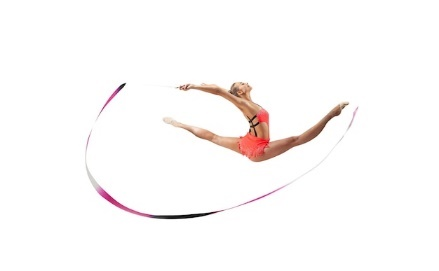
\includegraphics[width=1.98053in,height=1.22549in]{./imgs/img5.jpg}
\caption{Disponível em:
https://br.freepik.com/fotos-gratis/ginasta-ritmica-isolada-em-branco\_31843256.htm\#query=gin\%C3\%A1stica\%20art\%C3\%ADstica\&position=41\&from\_view=search\&track=ais.}
\end{figure}

A capacidade física utilizada no esporte apresentado é a

\begin{escolha}
\item força, pois a atleta está realizando um movimento com uma sobrecarga.

\item flexibilidade, pois a atleta está realizando uma abertura total das
pernas.

\item velocidade, pois a atleta deve se movimentar rapidamente a fita.

\item resistência, pois a atleta está saltando o mais alto que conseguir
\end{escolha}

\coment{Saeb: Identificar as diferentes valências físicas necessárias à
realização de práticas corporais (jogos eletrônicos, lutas, práticas
corporais de aventura, ginásticas, esportes e dança).

BNCC: (EF89EF03):~formular e utilizar estratégias para solucionar os
desafios técnicos e táticos, tanto nos esportes de campo e taco,
rede/parede, invasão e combate como nas modalidades esportivas
escolhidas para praticar de forma específica.

a) Incorreta. Porque a fita da ginástica é leve e não é considerada como
uma sobrecarga;
b) Correta. Porque a flexibilidade consiste da pessoa alongar (esticar)
ao máximo uma musculatura;
c) Incorreta. Porque a capacidade física da velocidade consiste da
pessoa realizar um movimento rápido, e não a fita da ginástica;
d) Incorreta. Porque a resistência consiste na pessoa realizar o mesmo
movimento por várias vezes, e não em saltar mais alto.}

\num{2} Leia o texto a seguir:

\begin{quote}
A tarde da última sexta foi um dia histórico para os skatistas
valadarenses isso porque na ocasião a classe não só recebeu a notícia de
que a pista de skate da Feira da Paz será reformada como também pôde
falar sobre suas expectativas, discutir e sugerir propostas para o
projeto. {[}...{]}

O publicitário e skatista Diogo Lage foi à luta, procurou e indicou a
empresa especializada em pistas de skate para a SMCELT, levou o
arquiteto responsável pela elaboração dos projetos nas pistas e agora
está confiante. ``Com a reforma e revitalização do espaço as famílias
poderão voltar a frequentar o local levando as crianças e a comunidade
terá oportunidade de conhecer melhor o mais novo esporte olímpico. Com o
projeto concluído os skatistas e o coletivo valadarense de skate fará a
Escolinha Social de Skate, que será uma oportunidade para tirar os
jovens do risco social da violência''.

\fonte{Prefeitura vai reformar a pista de skate. Prefeitura de Governador
Valadares. Disponível em:
https://www.valadares.mg.gov.br/detalhe-da-materia/info/prefeitura-vai-reformar-a-pista-de-skate/170101.
Acesso em: 22 fev. 2023.}
\end{quote}

Com base no texto, o projeto da cidade tem o objetivo de

\begin{escolha}
\item incentivar a prática de esportes urbanos.

\item formar atletas olímpicos.

\item atrair novos investidores.

\item criar um espaço restrito para um grupo social.
\end{escolha}

\coment{Saeb: Identificar o valor do patrimônio urbano e natural nas vivências
das práticas corporais de aventura urbana e na natureza.

BNCC: (EF67EF06):~analisar as transformações na organização e na prática
dos esportes em suas diferentes manifestações (profissional e
comunitário/lazer).

a) Correta. Porque o texto fala que o projeto é restruturação da pista
de skate da cidade para que mais pessoas possam praticar um esporte;
b) Incorreta. Porque o objetivo do projeto é ter novos praticantes, e
não novos atletas;
c) Incorreta. Porque o projeto da pista é para incentivar a pratica de
esportes;
d) Incorreta. Por mais que a pista é voltada para os skatistas, o texto
fala que é um local público para toda a comunidade.}

\num{3}  Leia a reportagem a seguir:

\begin{quote}
Respeito e disciplina são a base de tudo. As outras regras que você
precisa saber para acompanhar o judô estão aqui.

\textbf{Tatame}\\
As lutas acontecem em um tatame quadrado, com medidas que variam de 14 a
16 metros.

\textbf{Uniforme}\\
Os judocas devem usar um quimono. Um dos atletas recebe uma faixa
vermelha, além da própria faixa, e é chamado de aka (vermelho). O outro
recebe uma faixa branca e é chamado de shiro (branco).

\textbf{Duração} da luta\\
As lutas têm duração de 4 minutos para o feminino sênior e sub-21, e de
5 minutos para o masculino sênior.

\fonte{Regras. Infraero. Disponível em:
http://www.infraero.gov.br/judo/regras/. Acesso em: 22 fev. 2023.}
\end{quote}

Podemos perceber que o judô passou por um processo de esportivização,
pois nessa luta

\begin{escolha}
\item tem categorias masculinas e femininas

\item deve ser usado quimonos para competir.

\item existem regras e vestimentas padronizadas.

\item apresenta valores éticos e morais.
\end{escolha}

\coment{Saeb: Identificar as características (códigos, rituais, elementos
técnico-táticos, indumentária, materiais, instalações, instituições) das
lutas.

BNCC: (EF89EF18):~discutir as transformações históricas, o processo de
esportivização e a midiatização de uma ou mais lutas, valorizando e
respeitando as culturas de origem.

a) Incorreta. Porque ter categorias masculinas e femininas não define
que uma luta é um esporte oficial, apenas que a luta é difundida;
b) Incorreta. Porque o quimono é uma vestimenta usada no judô por causa
da sua origem cultural japonesa;
c) Correta. Porque uma luta esportivizada consiste em padronizar as
regras para as competições, como é mostrado no texto;
d) Incorreta. Porque respeito e disciplina são elementos culturais do
judô e não do esporte.}

\chapter{Simulado 2}

\num{1} Leia o texto a seguir

\begin{quote}
O Ministério da Educação, por meio do Fundo Nacional de Desenvolvimento
da Educação (FNDE), tem liberado recursos para a construção de 6.116
quadras esportivas {[}...{]}

``Essa quadra foi um presente para a escola e para a comunidade'',
comemora a diretora Socorro Lima da Silva. Segundo ela, duas vezes por
semana alunos da Escola Municipal Walmik Sampaio de Albuquerque utilizam
a quadra da escola Vinícius de Morais para as aulas de educação física.
``Durante a semana, de 17h às 20h, a quadra é utilizada pela comunidade,
em jogos de futsal. E, nos fins de semana, é utilizada em atividades do
programa Escola Aberta, como eventos religiosos'', explica.

\fonte{Escolas devem ser indicadas até setembro para ter quadras. Ministério da
Educação. Disponível em:
http://portal.mec.gov.br/ultimas-noticias/384-fnde-1801140772/18039-escolas-devem-ser-indicadas-ate-setembro-para-ter-quadras.
Acesso em: 22 fev. 2023.}
\end{quote}

Depois de ler o texto, as quadras esportivas tem como função de

\begin{escolha}
\item aumentar recursos financeiros da cidade.

\item incentivar a pratica de esportes.

\item promover competições oficiais de diferentes modalidades.

\item ser utilizada prioritariamente para os alunos da escola municipal.
\end{escolha}

\coment{Saeb: Analisar as práticas corporais frente à disponibilidade de locais
para sua vivência.

BNCC: (EF89EF03):~formular e utilizar estratégias para solucionar os
desafios técnicos e táticos, tanto nos esportes de campo e taco,
rede/parede, invasão e combate como nas modalidades esportivas
escolhidas para praticar de forma específica.

a) Incorreta. Porque as quadras esportivas servem para promover a
pratica de espores, e não de trazer mais recursos financeiros;
b) Correta. Porque as quadras esportivas, com base no texto, são espaços
públicos para que a população da cidade use para realizar esportes;
c) Incorreta. Porque o texto não menciona que as quadras servem para as
competições, e sim para praticar algum esporte;
d) Incorreta. Porque as quadras são destinadas para toda a comunidade da
escola.}

\num{2} Leia o texto a seguir:

\begin{quote}
Para os povos da Antiguidade, o manuseio da espada era fundamental,
tendo em vista as constantes guerras e batalhas travadas.~ {[}...{]}

A Federação Internacional de Esgrima só foi criada em 1913. O primeiro
Campeonato Mundial da modalidade aconteceu em 1921, em Paris. Mas a
história da esgrima nos Jogos Olímpicos começou antes. Já em Atenas-1896
houve provas do esporte. Desde então, a esgrima nunca deixou de estar
presente em uma edição das Olimpíadas.

\fonte{Esgrima. Rede do Esporte. Disponível em:
http://rededoesporte.gov.br/pt-br/megaeventos/olimpiadas/modalidades/esgrima-1.
Acesso em: 22 fev. 2023.}
\end{quote}

Após a leitura do texto, a esgrima se tornou um esporte oficial pelo fato de

\begin{escolha}
\item fazer parte dos jogos olímpicos.

\item ter órgãos oficiais.

\item ser usada em guerras.

\item usar um implemento para competir.
\end{escolha}

\coment{Saeb: Analisar as transformações históricas, o processo de
esportivização e a midiatização das práticas corporais, com ênfase nas
lutas.

BNCC: (EF89EF18):~discutir as transformações históricas, o processo de
esportivização e a midiatização de uma ou mais lutas, valorizando e
respeitando as culturas de origem.

a) Incorreta. Porque o fato de uma luta fazer parte das Olimpíadas não
caracteriza como um processo de esportivização;
b) Correta. Porque uma luta para ser uma modalidade oficial, é
necessário ter federações ou confederações oficiais;
c) Incorreta. Porque a luta ser usada para guerra não quer dizer que é
um esporte oficial;
d) Incorreta. Porque o uso da espada é uma característica da esgrima e
não de um esporte de combate oficial.}

\num{}  Leia a reportagem a seguir.

\begin{quote}
O Breaking Dance é um estilo que foi inserido recentemente entre as
modalidades das Olimpíadas e integrará os próximos jogos de Paris, na
França, em 2024. O tema~vem movimentando as comunidades de danças
urbanas em todo o Brasil, esquentando o debate sobre a legitimidade do
Break como modalidade olímpica, tendo em vista~ser considerado,
originalmente, um estilo de dança da cultura Hip Hop.

\fonte{Painel Funesc de dança traz debate sobre o Break Dance nas Olimpíadas.
Governo da Paraíba. Disponível em:
https://paraiba.pb.gov.br/noticias/painel-funesc-de-danca-traz-debate-sobre-o-break-dance-nas-olimpiadas.
Acesso em: 22 fev. 2023.}
\end{quote}

Com base no texto, podemos compreender que o break

\begin{escolha}
\item criou a cultura do hip-hop.

\item passou a se tornar um esporte.

\item incentivou as competições de dança.

\item perdeu suas características das danças urbanas.
\end{escolha}

\coment{Saeb: Diferenciar os esportes com base nos critérios de sua lógica
interna.

BNCC: (EF67EF13):~diferenciar as danças urbanas das demais manifestações
da dança, valorizando e respeitando os sentidos e significados
atribuídos a eles por diferentes grupos sociais.

a) Incorreta. Porque foi a cultura do hip-hop que criou o break e outras
práticas corporais;
b) Correta. Porque o break vai fazer parte de uma competição oficial
(Olimpíadas), portanto podemos considerar essa dança como um esporte
oficial;
c) Incorreta. Porque a dança urbana não incentivou as competições,
apenas foi inserida nos jogos olímpicos;
d) Incorreta. Porque as características do break se mantem, como ritmo,
gestos etc., apenas vai ter regras padronizadas para as olimpíadas.}

\chapter{Simulado 3}

\num{1}  Leia o texto a seguir:

\begin{quote}
Na condição de cultura urbana, o Hip Hop surgiu na periferia de Nova
York, entre as comunidades caribenhas, afro-americanas e
latino-americanas na década de 1970. O contexto social era de violência
e criminalidade nesses bairros, e a única forma de lazer possível para
os jovens era nas ruas. Encontraram na música, poesia, dança e na
pintura uma forma de manifestação de sua realidade e contestação.

\fonte{Iniciação ao Hip Hop desperta interesse dos adolescentes no Projeto
``Danças Urbanas''. Governo do Estado do Ceará. Disponível em:
https://www.seas.ce.gov.br/2021/08/05/iniciacao-ao-hip-hop-desperta-interesse-dos-adolescentes-no-projeto-dancas-urbanas/\#:\textasciitilde{}:text=Origem\%20do\%20Hip\%20Hop,os\%20jovens\%20era\%20nas\%20ruas.
Acesso em: 22 fev. 2023.}
\end{quote}

Após ler a reportagem, o hip-hop surgiu com o objetivo de

\begin{escolha}
\item incentivar a pratica esportiva em espaços abertos.

\item incluir a participação de novos grupos sociais.

\item diminuir a violência na cidade.

\item realizar protesto de maneira pacifica.
\end{escolha}

\coment{Saeb: Diferenciar as danças urbanas, seus elementos constitutivos e seu
valor cultural nas demais manifestações da dança.

BNCC: (EF67EF12):~planejar e utilizar estratégias para aprender
elementos constitutivos das danças urbanas.

a) Incorreta. Porque no hip-hop as pessoas realizavam danças e não
esportes;
b) Incorreta. Porque o hip-hop surgiu por causa de uma minoria que vivia
nos Estados Unidos, ou seja, eles eram excluídos;
c) Incorreta. Porque o hip-hop não diminuiu a violência, apenas usava a
dança e as músicas como forma de protesto;
d) Correta. Porque no hip-hop as pessoas usavam o rap, a dança e o
grafite como formar de mostrar para a sociedade as situações deles de
uma maneira pacifica.}

\num{2}  Leia o texto a seguir:

\begin{quote}
Segundo
o Blog da Saúde, a vigorexia é um tipo de transtorno dismorfóbico -- de
distorção da autoimagem {[}...{]}

Desse modo, a vigorexia é uma doença psicológica caracterizada pela
insatisfação constante com o corpo {[}...{]}

\fonte{Precisamos falar do excesso de atividade física: você sabe o que é
vigorexia? Ministério da Saúde. Disponível em:
https://www.gov.br/saude/pt-br/assuntos/saude-brasil/eu-quero-me-exercitar/noticias/2021/precisamos-falar-do-excesso-de-atividade-fisica-voce-sabe-o-que-e-vigorexia.
Acesso em: 22 fev. 2023.}
\end{quote}

Uma prática comum da pessoa que tem vigorexia é

\begin{escolha}
\item ter uma preocupação exagerada com a alimentação.

\item treinar exercícios físicos em excesso.

\item induzir o vômito após uma refeição.

\item comer pequenas quantidades de alimentos.
\end{escolha}

\coment{Saeb: Avaliar a multiplicidade de padrões de estética corporal
disseminados pela mídia, que geram uma prática excessiva de exercícios e
o uso de recursos ergogênicos

BNCC: (EF89EF08):~discutir as transformações históricas dos padrões de
desempenho, saúde e beleza, considerando a forma como são apresentados
nos diferentes meios (científico, midiático, etc.).

a) Incorreta. Porque a definição apresentada é da ortorexia;
b) Correta. Porque pessoas com vigorexia se enxergam com pouco volume
muscular e treinam de maneira excessiva para ter mais hipertrofia
muscular;
c) Incorreta. Porque são as pessoas com bulimia que induzem o vômito;
d) Incorreta. Porque diminuir a quantidade de alimentos é uma
característica de uma pessoa com anorexia.}

\num{3}  Leia o texto a seguir

\begin{quote}
Doping refere-se ao uso de substâncias naturais ou sintéticas {[}...{]}
Este objetivo é ilícito e por isso são feitos testes de doping durante
competições.

\fonte{Doping. Secretaria da Educação. Disponível em:
http://www.ciencias.seed.pr.gov.br/modules/galeria/detalhe.php?foto=1845\&evento=1.
Acesso em: 22 fev. 2023.}
\end{quote}

Após ler o texto, os atletas que são pegos do doping são aqueles que

\begin{escolha}
\item evitam o uso de substâncias ilegais.

\item usam medicamentos proibidos para ganhar as competições.

\item ingerem substâncias para se igualar aos demais competidores.

\item aplicam os anabolizantes para cuidar da saúde.
\end{escolha}

\coment{Saeb: Avaliar os problemas presentes nos esportes e abordados pela
mídia, tais como doping, violência ou corrupção.

BNCC: (EF89EF09):~problematizar a prática excessiva de exercícios
físicos e o uso de medicamentos para a ampliação do rendimento ou
potencialização das transformações corporais.

a) Incorreta. Porque atletas que são pegos no doping fazem usam de
substâncias ilegais;
b) Correta. Porque alguns atletas usam substâncias ilegais com o
objetivo de ganhar a qualquer custo;
c) Incorreta. Porque o uso de sustâncias pode potencializar o despenho
do atleta causando uma desigualdade entre os competidores;
d) Incorreta. Porque o uso de anabolizantes para alguns atletas não é
para a saúde e sim para ganhar as competições.}

\chapter{Simulado 4}

\num{1} Leia o texto a seguir:

\begin{quote}
A atividade física é importante para o pleno desenvolvimento humano e
deve ser praticada em todas as fases da vida e em diversos momentos.
Além de apresentar inúmeros benefícios para a proteção e prevenção de
Doenças Crônicas Não Transmissíveis (DCNTs), a prática também tem
influência positiva nos aspectos psicológicos e sociais. Isso porque
muitas atividades coletivas incentivam a socialização, sendo esse um
elemento importante para todos, principalmente para crianças e
adolescentes, como parte da formação, assim como é um poderoso estímulo
para pessoas idosas.

\fonte{Conheça o primeiro Guia de Atividade Física para a População Brasileira.
Ministério da Saúde. Disponível em:
https://www.gov.br/saude/pt-br/assuntos/saude-brasil/eu-quero-me-exercitar/noticias/2021/conheca-o-primeiro-guia-de-atividade-fisica-para-a-populacao-brasileira.
Acesso em: 22 fev. 2023.}
\end{quote}

Após ler o texto, podemos afirmar que as atividades físicas tem como
propósito de

\begin{escolha}
\item incentivar práticas corporais individuais pra melhor o aspecto
social.

\item promover a saúde e qualidade de vida.

\item priorizar benefícios pra um grupo de pessoas.

\item diminuir benefícios relacionados aos aspectos mentais.
\end{escolha}

\coment{Saeb: Avaliar a relação entre as práticas corporais e a promoção da
saúde.

BNCC: (EF89EF08):~discutir as transformações históricas dos padrões de
desempenho, saúde e beleza, considerando a forma como são apresentados
nos diferentes meios (científico, midiático, etc.).

a) Incorreta. Porque o texto fala que as atividades físicas realizadas
coletivamente trazem benefícios sociais;
b) Correta. Porque a prática regular de atividades físicas evita o
desenvolvimento de doenças;
c) Incorreta. Porque as atividades físicas trazem benefícios para todos
os grupos sociais;
d) Incorreta. Porque as atividades trazem inúmeros benefícios no aspecto
mental e psicológico para as pessoas.}

\num{2}  Leia a reportagem a seguir:

\begin{quote}
Iniciam amanhã, os Jogos Escolares Eletrônicos do Paraná. A 2ª~edição da
competição~acontecerá em 5 finais de semana nos meses de setembro e
outubro. A introdução do e-sports nos Jogos Oficiais do Estado aconteceu
ano passado visando o intercâmbio, e o entretenimento, aproximando os
alunos como forma de atenuar os efeitos nocivos causados pela pandemia
da Covid-19.~{[}...{]}

Para a coordenadora dos Jogos Escolares do Paraná, Márcia Tomadon,
"tomamos esta medida~para que todos os alunos possam participar. Muitas
vezes as escolas não conseguem montar uma equipe, então desta maneira
damos a possibilidade de todos estarem contemplados na competição, e
assim também já conseguimos uma interação entre crianças de escolas
diferentes". Ela também ressaltou o bom número de alunos inscritos:
"foram~2.742 inscrições, um bom número tendo em vista que estamos
introduzindo o e-sports na cultura esportiva-escolar".~

\fonte{Jogos Escolares Eletrônicos tem início neste sábado. Paraná Esporte.
Disponível em:
https://www.esporte.pr.gov.br/Noticia/Jogos-Escolares-Eletronicos-tem-inicio-neste-sabado.
Acesso em: 22 fev. 2023.}
\end{quote}

Depois de ler a reportagem, podemos afirmar que os e-sports

\begin{escolha}
\item são utilizados para evitar a pandemia.

\item podem ser considerados como esporte por possuírem competições
oficiais.

\item ajudam na formação de atletas de jogos eletrônicos

\item promove malefícios para os praticantes.
\end{escolha}

\coment{Saeb: Identificar as diferentes valências físicas necessárias à
realização de práticas corporais (jogos eletrônicos, lutas, práticas
corporais de aventura, ginásticas, esportes e dança).

BNCC: (EF67EF01):~experimentar e fruir, na escola e fora dela, jogos
eletrônicos diversos, valorizando e respeitando os sentidos e
significados atribuídos a eles por diferentes grupos sociais e etários.

a) Incorreta. Porque a competição citada foi criada durante a pandemia
por conta do isolamento social e não para acabar com a pandemia;
b) Correta. Porque um esporte oficial é quando tem competições oficiais,
como os Jogos Escolares Eletrônicos;
c) Incorreta. Porque a competição citada no texto é para promover a
participação dos alunos e não para ter novos atletas de alto rendimento;
d) Incorreta. Porque no texto fala que os jogos eletrônicos promovem a
socialização por meio de interações dos jogos eletrônicos.}

\num{3}  Leia o texto a seguir:

\begin{quote}
Apesar de adorar dançar, Mara Raymundo começou a dançar como forma de
exercício físico para melhorar picos de pressão que tinha por conta da
vida agitada. "Não queria tomar remédio, então fui dançar e hoje tenho a
pressão normal", justifica Mara. Mas não foi só a pressão da Mara que
melhorou. "A memória melhorou, decorando os passos da dança, e a relação
com os outros também, além do humor, do sono e da disposição. Me sinto
como se tivesse 15 anos", comemora. Há um ano e meio ela dança duas
horas por dia, três vezes na semana, e ainda sai para dançar com os
amigos nos fins de semana. "A música eleva, inspira", completa.~ ~ ~

\fonte{Dançar faz bem ao corpo, à alma e à mente. Ministério da Saúde.
Disponível em:
https://www.gov.br/saude/pt-br/assuntos/saude-brasil/eu-quero-me-exercitar/noticias/2018/dancar-faz-bem-ao-corpo-a-alma-e-a-mente.
Acesso em: 22 fev. 2023.}
\end{quote}

Após ler a reportagem, podemos afirmar que a prática corporal citada

\begin{escolha}
\item ajudou a pessoa em ter uma rotina mais movimentada.

\item prejudicou o uso de medicamentos.

\item diminuiu o gasto de energia.

\item trouxe benefícios para o aspecto social.
\end{escolha}

\coment{Saeb: Avaliar a relação entre as práticas corporais e a promoção da
saúde.

BNCC: (EF89EF15):~analisar as características (ritmos, gestos,
coreografias e músicas) das danças de salão, bem como suas
transformações históricas e os grupos de origem.

a) Incorreta. Porque a dança fez com que a pressão alta diminuísse por
causa da vida agitada da praticante de dança;
b) Incorreta. Porque a dança fez com que a praticante diminuísse o uso
de medicamento, fazendo que isso se tornasse um benefício;
c) Incorreta. Porque realizar a dança com uma certa frequência na semana
faz com que a pessoa tenha mais gasto calórico (energia);
d) Correta. Porque no trecho ``...ela dança duas horas por dia, três
vezes na semana, e ainda sai para dançar com os amigos nos fins de
semana...'' é possível analisar que a dança ajudou na socialização.}


